This chapter introduces how to model interactions with multiple waveguides (or equivalently multiple waveguide modes) in the time-binned photon picture. We will show how this can be used to extend the simulations in chapter \ref{ch3} so that we are no longer restricted to only one propagating mode. We consider an emitter coupled to two directional waveguide modes and reproduce results from a recent experimental demonstration of two-photon scattering in photonic crystal waveguides \cite{LeJeannic2022DynamicalEmitter}. We also consider how to model direct interactions between waveguide modes. Such interactions can arise from scattering elements in the waveguide leading to e.g. a beamsplitter. We start by considering a fundamental Hamiltonian shown to obey flux conservation and time-reversal symmetry as required by input-output theory or in the classical limit: coupled mode theory. By discretizing the Hamiltonian into time bins, we find a discrepancy between the expected input-output relations and the discretized Hamiltonian. We investigate this discrepancy by considering the change in the lifetime of an emitter coupled to a waveguide with a scattering element. We find inconsistencies in the emitter lifetime found by the numerical approach but also show that these can be solved by an effective renormalization of the interaction strength between the emitter and waveguide modes. 
\begin{figure}[H]
    \centering
    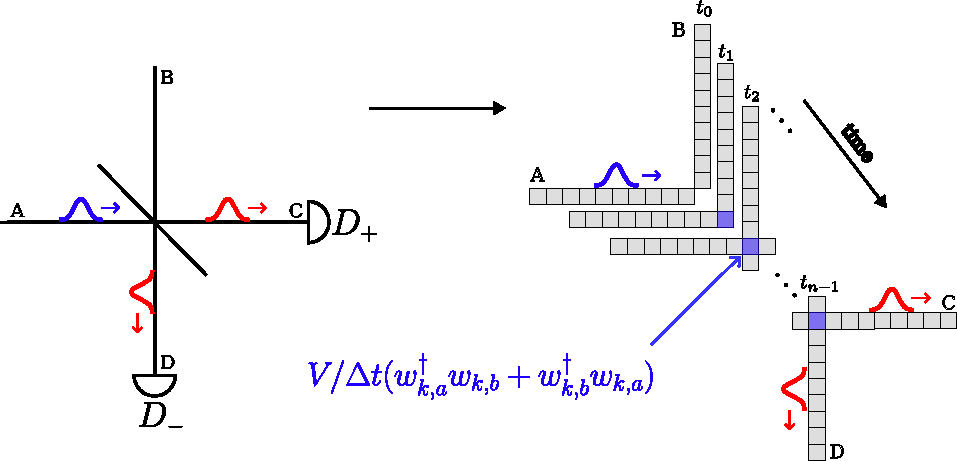
\includegraphics[width = \linewidth]{figures/waveguideinteraciton.pdf}
    \caption{Left: Sketch of a beamsplitter, where an incoming pulse (blue) scatters on the beamsplitter and is split into two identical output pulses (red). Right: Numerical representation of the interaction between binned photons in two waveguides. The initial state is defined at $t_0$, and when $t_n$ is reached, the two pulses have interacted and in the shown sketch the beamsplitter transformation has been performed. }
    \label{fig:beamsplitter_illustration}
\end{figure}


\section{Representing multiple waveguides efficiently }

Before we simulate the interactions with multiple waveguides, we will discuss how to represent them numerically. The naive approach is to define two waveguide bases, as introduced in chapter \ref{ch3}. However, a quick estimate of the total size of the Hilbert space reveals this approach to be infeasible. Suppose we want to describe two waveguide modes interfering on a beam splitter. Although the initial state only contains a single photon in each waveguide, we can have two photons in the waveguides after the interaction. Thus, we need two waveguide bases for modes $a$ and $b$, each containing up to two photons. If we take $N=100$, we thus have two Hilbert spaces each of size: $1+N+N(N+1)/2 = 5151$, meaning a combined Hilbert space of size: $5151^2 = 26.532.801$!!! Even with the LazyOperators and sparse representations, this is too large to be numerically feasible. Luckily, we can create a much more efficient storing strategy by realizing that we are storing unnecessary parts of the state vector. In this example, we only have a total of two excitations, meaning that states with two photons in each waveguide simultaneously are unobtainable, that is, states of the type: $\sum_{i,j,k,l}\xi^{(4)}(t_i,t_j,t_k,t_j) \ket{1_i,1_j}_a\ket{1_k,1_j}_b$, where the subscripts $a$ and $b$ denote waveguide modes $a$ and $b$, respectively. Therefore, if we restrict ourselves to states only containing at max two excitations, the Hilbert space reduces drastically in size. We are thus describing states with the general form:
\begin{align}
    \ket{\psi} &= \ket{\emptyset}_a\ket{\emptyset}_b + \sum_k \xi_a^{(1)}(t_k) \ket{1_k}_a\ket{\emptyset}_b + \sum_k \xi_b^{(1)}(t_k) \ket{\emptyset}_a\ket{1_k}_b + \sum_{k,l \geq k}\xi_a^{(2)}(t_k,t_j) \ket{1_k,1_j}_a \ket{\emptyset}_b \\ 
    &+ \sum_{k,l \geq k}\xi_b^{(2)}(t_k,t_j) \ket{\emptyset}_a \ket{1_k,1_j}_b+ \sum_{k,l}\xi_{a,b}^{(2)}(t_k,t_j) \ket{1_k}_a \ket{1_j}_b
\end{align}

\begin{figure}
    \centering
    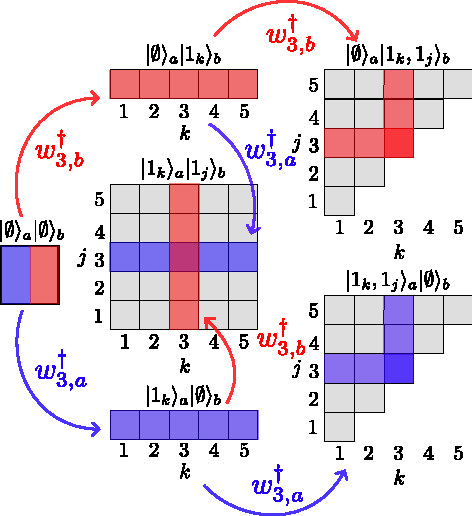
\includegraphics[width = 0.6 \linewidth]{figures/multiplewaveguides_illustration.pdf}
    \caption{Illustration of numerical representation of two waveguides containing two excitations. Blue colors are associated with creating a photon in waveguide $a$ and red with creating a photon in $b$. }
    \label{fig:twowaveguide_illustration}
\end{figure}

Notice that we now have a new two-time wavefunction $\xi^{(2)}_{a,b}(t_k,t_j)$ describing having a single-photon excitation simultaneously in waveguide $a$ and $b$. $\xi^{(2)}_{a,b}(t_k,t_j) = \xi^{(2)}_{a,b}(t_j,t_k)$ is in general not true, and we thus store a $N^2$ matrix to represent this state. An illustration of the total state of two waveguides containing two excitations can also be seen in Fig. \ref{fig:twowaveguide_illustration}. Here, we also show the effect of acting with the creation operators $w^\dagger_{3,a/b}$, where all blue lines are associated with creating a photon in waveguide mode $a$ and red lines with creating photons in waveguide mode $b$. Our Hilbert space is now of size $1+N+2 N(N+1)/2 + N^2 = 20201$, thus three orders of magnitude smaller than the initial naive approach!






\section{Scattering On a Single Emitter \label{sec:lodahl}}
\begin{figure}[H]
    \centering
    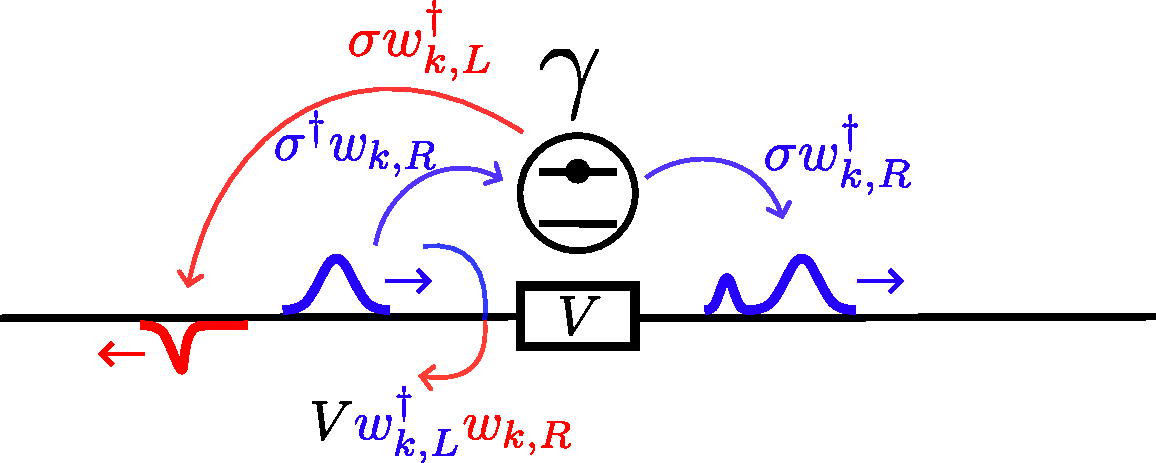
\includegraphics[width=\linewidth]{figures/lodahl_waveguide.pdf}
    \caption{Illustration of a right propagating excitation (blue) in a waveguide coupled to a two-level system with the factor $\gamma$. After the blue pulse has scattered, there is also an excitation going to the left (red). A coupling between the left and right propagating modes $V$ is also shown, which can be thought of as a partially transmitting mirror in the waveguide.}
    \label{fig:lodahl_sketch}
\end{figure}

With an effective representation of multiple waveguides, we can now simulate an emitter coupled to multiple waveguide modes. In fig. \ref{fig:lodahl_sketch} we show a waveguide with two directionally propagating modes (left and right) coupled to a two-level system with the rate $\gamma$. In the waveguide, we have also placed a partially transmitting mirror (PTE) which couples the left and right propagating modes with each other with a strength $V$. We will discuss this PTE and how to model it in detail in later sections. For now, the scattering element is completely transparent and the Hamiltonian for this configuration is:
\begin{equation}
    H = i \sqrt{\gamma_\mathrm{L}/\Delta t} ( \sigma^\dagger w_{k,\mathrm{L}} - \sigma w^\dagger_{k,\mathrm{L}} ) + i \sqrt{\gamma_\mathrm{R}/\Delta t} ( \sigma^\dagger w_{k,\mathrm{R}} - \sigma w^\dagger_{k,\mathrm{R}})  \label{eq:lodahl_ham}
\end{equation}
Here, we have introduced subscripts $\mathrm{R}$ and $\mathrm{L}$ to denote right and left propagating excitations. $\gamma_i$ denotes the coupling to waveguide $i$, which we assume in the following to be symmetric $\gamma_R = \gamma_L = \gamma$. This system is studied theoretically in ref. \cite{Joanesarson2020Few-photonGeometries} and experimentally in ref. \cite{LeJeannic2022DynamicalEmitter}, where a quantum dot is placed in a photonic crystal waveguide.
\begin{listing}[H]
\begin{minted}[
frame=lines,
framesep=2mm,
baselinestretch=1.2,
bgcolor=LightGray,
fontsize=\small,
linenos,
escapeinside=||,
mathescape=true
]{julia}
#Define basis
times = 0:0.1:10
be = FockBasis(1)
bw = WaveguideBasis(2,2,times)

#Define operators for interacting with emitter
swdR = create(bw,1) |$\otimes$| destroy(be)
sdwR = destroy(bw,1) |$\otimes$| create(be)
swdL = create(bw,2) |$\otimes$| destroy(be)
sdwL = destroy(bw,2) |$\otimes$| create(be)

#Setup Hamiltonian
|$\gamma R$|,|$\gamma L$| = 1,1
H = im*sqrt(|$\gamma R$|/dt)*(sdwL-swdL) + im*sqrt(|$\gamma R$|/dt)*(sdwR-swdR)

#Initial state
w=1 #width of gaussian pulse
psi_in_two = twophoton(bw,1,xi2,w,w,t0) |$\otimes$| fockstate(be,0)
psi_in_single = onephoton(bw,1,xi,w,t0) |$\otimes$| fockstate(be,0)
\end{minted}
\caption{Code for simulating scattering of emitter coupled to two channels. In lines 1-3, we define the bases used. Lines 7-10 define $\sigma w^\dagger_{k,\mathrm{R}/\mathrm{L}}$, and lines 13-14 combine the operators to define the Hamiltonian. In line 18, we define the initial two-photon state, and in line 19 the single-photon state. \code{xi} and \code{xi2} are Gaussian functions as also defined in code sample \ref{ls:twophoton_scattering} and studied in Fig. \ref{fig:twophoton_detuning} and \ref{fig:twophoton_emitter_detuning}. }
\label{ls:lodahlcode}
\end{listing}

In the following, we show that with the Hamiltonian in eq. \eqref{eq:lodahl_ham}, we can reproduce the results of the experiment in ref. \cite{LeJeannic2022DynamicalEmitter}, where the difference between scattering a two-photon pulse or a one-photon pulse on an emitter in a waveguide is considered. In Code Sample \ref{ls:lodahlcode}, we define the system's Hamiltonian and the initial state in the WaveguideQED.jl framework \textcolor{red}{(Code could be excluded)}. We also define two initial states; a single-photon Gaussian pulse and a two-photon Gaussian pulse, as studied previously in chapter \ref{ch3}. In Fig. \ref{fig:lodahlfig2}, we vary the pulse width $\sigma$ and plot the transmitted two-photon wavefunction $\xi_{\mathrm{tt}}^{(2)}(t_1,t_2)$, where the subscripts $t$ here denotes that both photons are propagating in a transmitted state. For the two-photon state, this of course the right propagating state after the interaction: $\xi_{\mathrm{tt}}^{(2)}(t_1,t_2) = \xi_{\mathrm{RR}}^{(2)}(t_1,t_2)$. In ref. \cite{LeJeannic2022DynamicalEmitter}, the scattered two-photon wavefunction is shown to factorize as $\xi_{\mathrm{RR}}^{(2)}(t_1,t_2) = \xi_\mathrm{R}^{(1)}(t_1)\xi_\mathrm{R}^{(1)}(t_2) + N(t_1,t_2)$, where $\xi_\mathrm{R}^{(1)}(t_1)$ denotes the single-photon scattered wavefunction and $N(t_1,t_2)$ describes the non-linear interaction between the two-photon pulse and the emitter. We can thus characterize the effect of this non-linearity by considering the single-photon product state 
 $\xi_{\mathrm{tt}}^{(2)}(t_1,t_2) = \xi_\mathrm{R}^{(1)}(t_1)\xi_\mathrm{R}^{(1)}(t_2)$ corresponding to measuring correlations between two separate single-photon pulses. 



In fig. \ref{fig:lodahlfig2}, the single-photon product state and two-photon wavefunction are seen to be similar for narrow pulses. The emitter is unable to interact with the pulse effectively due to its short duration, and no appreciative non-linearity arises. As the width increases, a distinct difference, however, emerges. Similar to the scattering of the cavity, destructive interference leads to a reflection of the single-photon pulse, thus leading to a cross-like structure. For the two-photon pulse, we, however, have stimulated emission, which initially leads to a bird-like structure. For an even larger width $\sigma = 5$, the diagonal shape indicates that the two photons arrive almost exclusively as a pair, showing a strong temporal correlation due to stimulated emission. 

\begin{figure}[H]
    \centering
    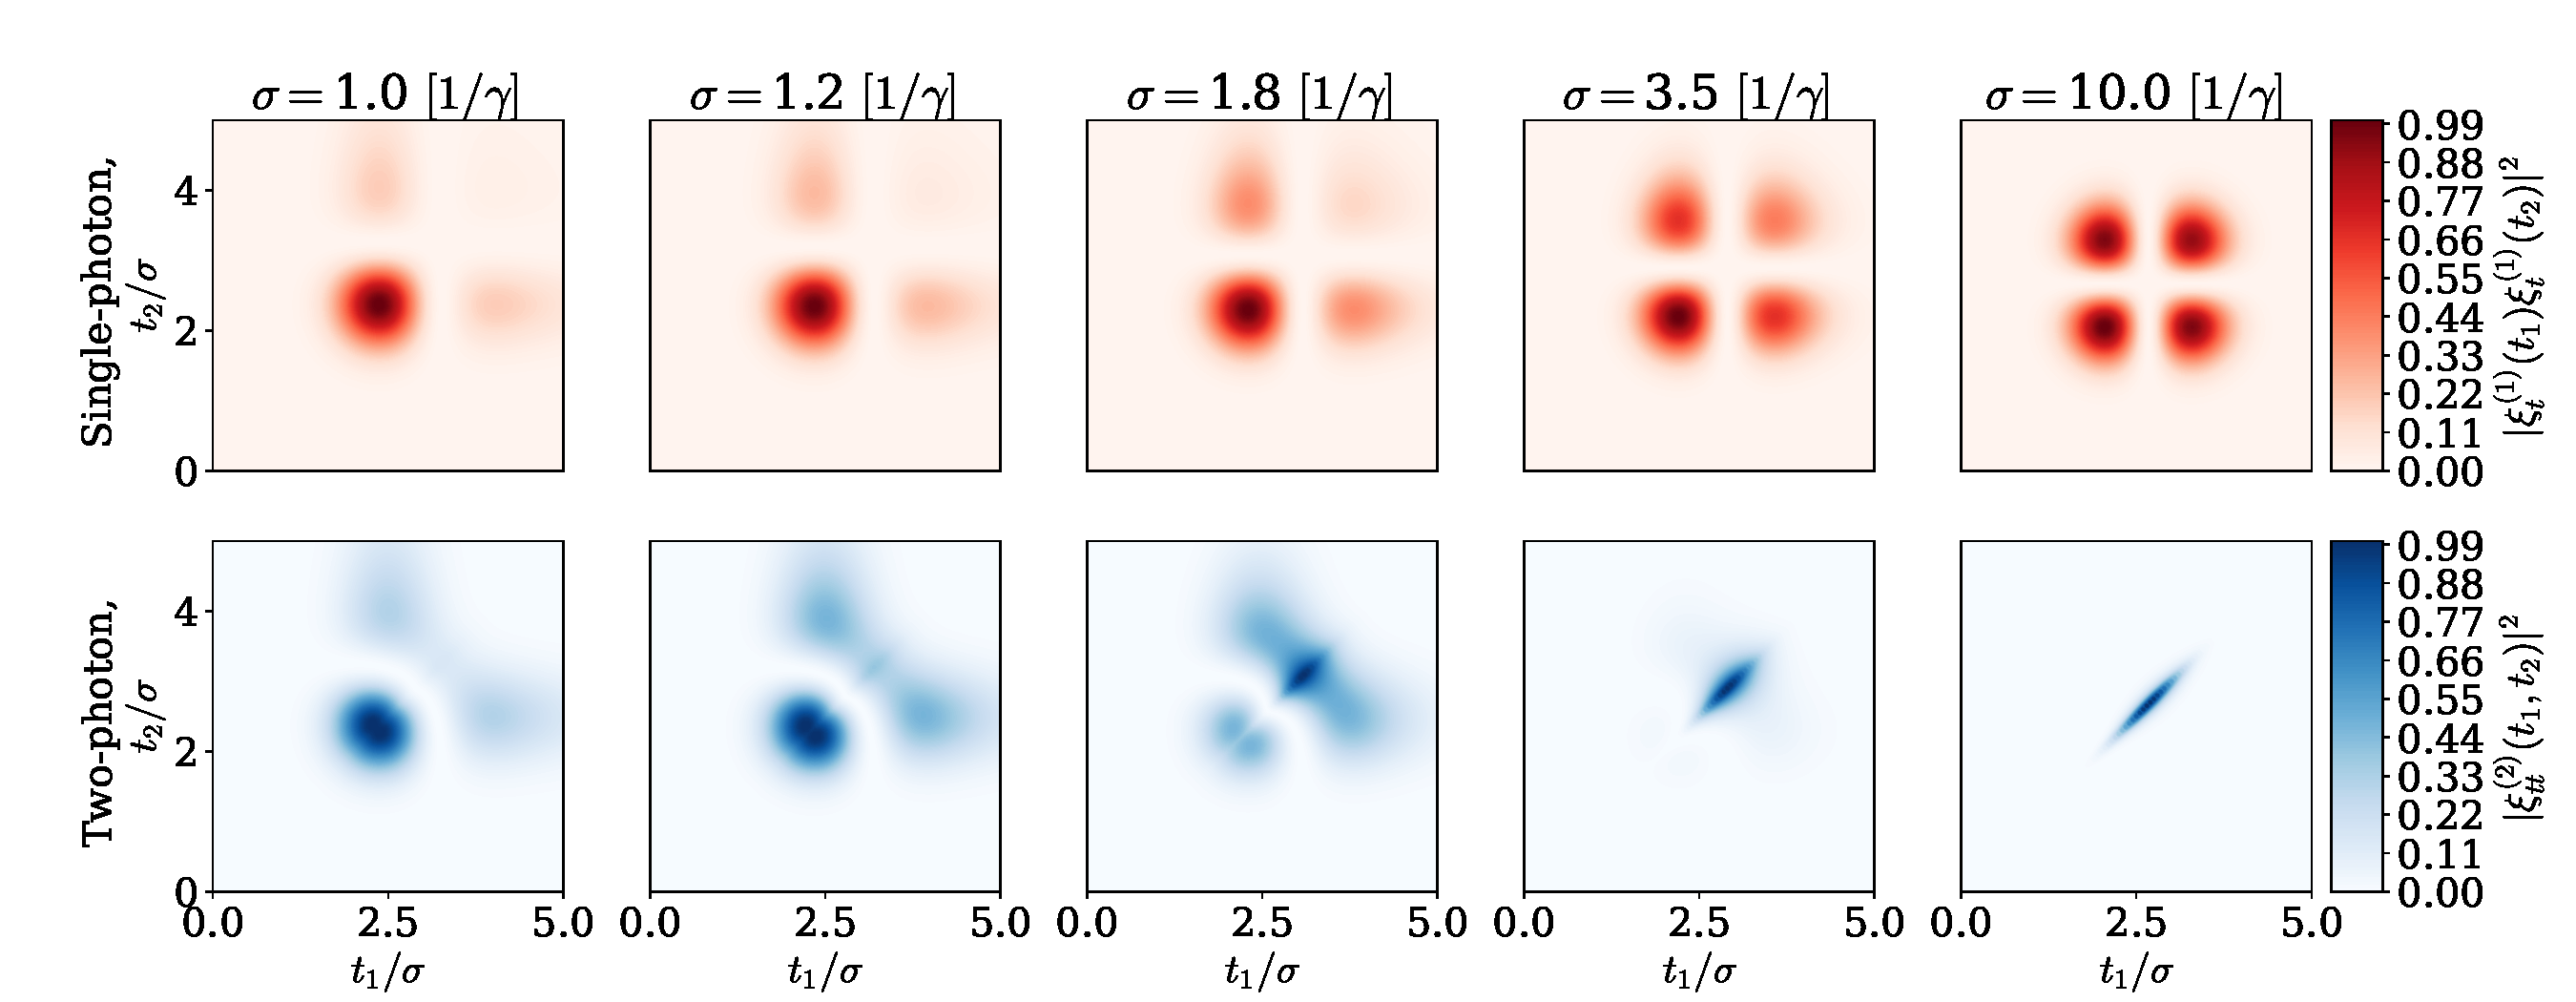
\includegraphics[width=\linewidth]{figures/lodahl_fig2.pdf}
    \caption{Upper panel (red): The product of two transmitted one-photon wavefunctions $|\xi_t^{(1)}(t_1)\xi_t^{(1)}(t_2)|^2$ from a single-photon Gaussian input state for varying widths of the Gaussian pulse $\sigma$. Lower panel (blue): Same as the upper panel but for a two-photon Gaussian input state. For ease of comparison, all contour plots have been normalized by dividing with largest value: $\mathrm{max}(|\xi_t^{(1)}(t_1)\xi_t^{(1)}(t_2)|^2)$ and $\mathrm{max}(|\xi_{tt}^{(2)}(t_1,t_2)$, respectively. \label{fig:lodahlfig2}}
\end{figure}

So far, this is all qualitatively very similar to the scattering of the emitter in the single-sided case. However, a clear distinction is seen if we consider not only the transmitted wavefunction but also the reflected wavefunction $\xi^{(2)}_{rr}$ (thus occupying the left propagating mode after the scattering) and partially reflected partially transmitted wavefunction $\xi^{(2)}_{rt}$. Here, $\xi^{(2)}_{rt}$ describes the amplitude of one photon in the reflected mode and one photon in the transmitted mode $\ket{1_i}_r\ket{1_j}_t$. In Fig. \ref{fig:lodahlfig3}, we show these three scattered wavefunctions for a single-photon and two-photon Gaussian pulse for a width $\sigma = 1$. In the two-photon case, the reflected wavefunction $\xi^{(2)}_{rr}$ shows a dip along the diagonal, showing that two photons cannot be reflected simultaneously. This is exactly the opposite case of the transmitted wavefunction, where stimulated emission leads to simultaneous photon emission and, thus, a strong diagonal.

In the single-photon pulse, there is no dip in the diagonal as the separate pulses are both able to be reflected. As for the two-photon partially reflected, partially transmitted wavefunction, we see a highly asymmetric wavefunction, showing the time-ordering of the process: We will not see a photon in the reflected channel if we did not first observe a photon in the transmitted channel. For the single-photon pulse, no such restriction occurs because we are here comparing two separate pulses.




\begin{figure}[H]
    \centering
    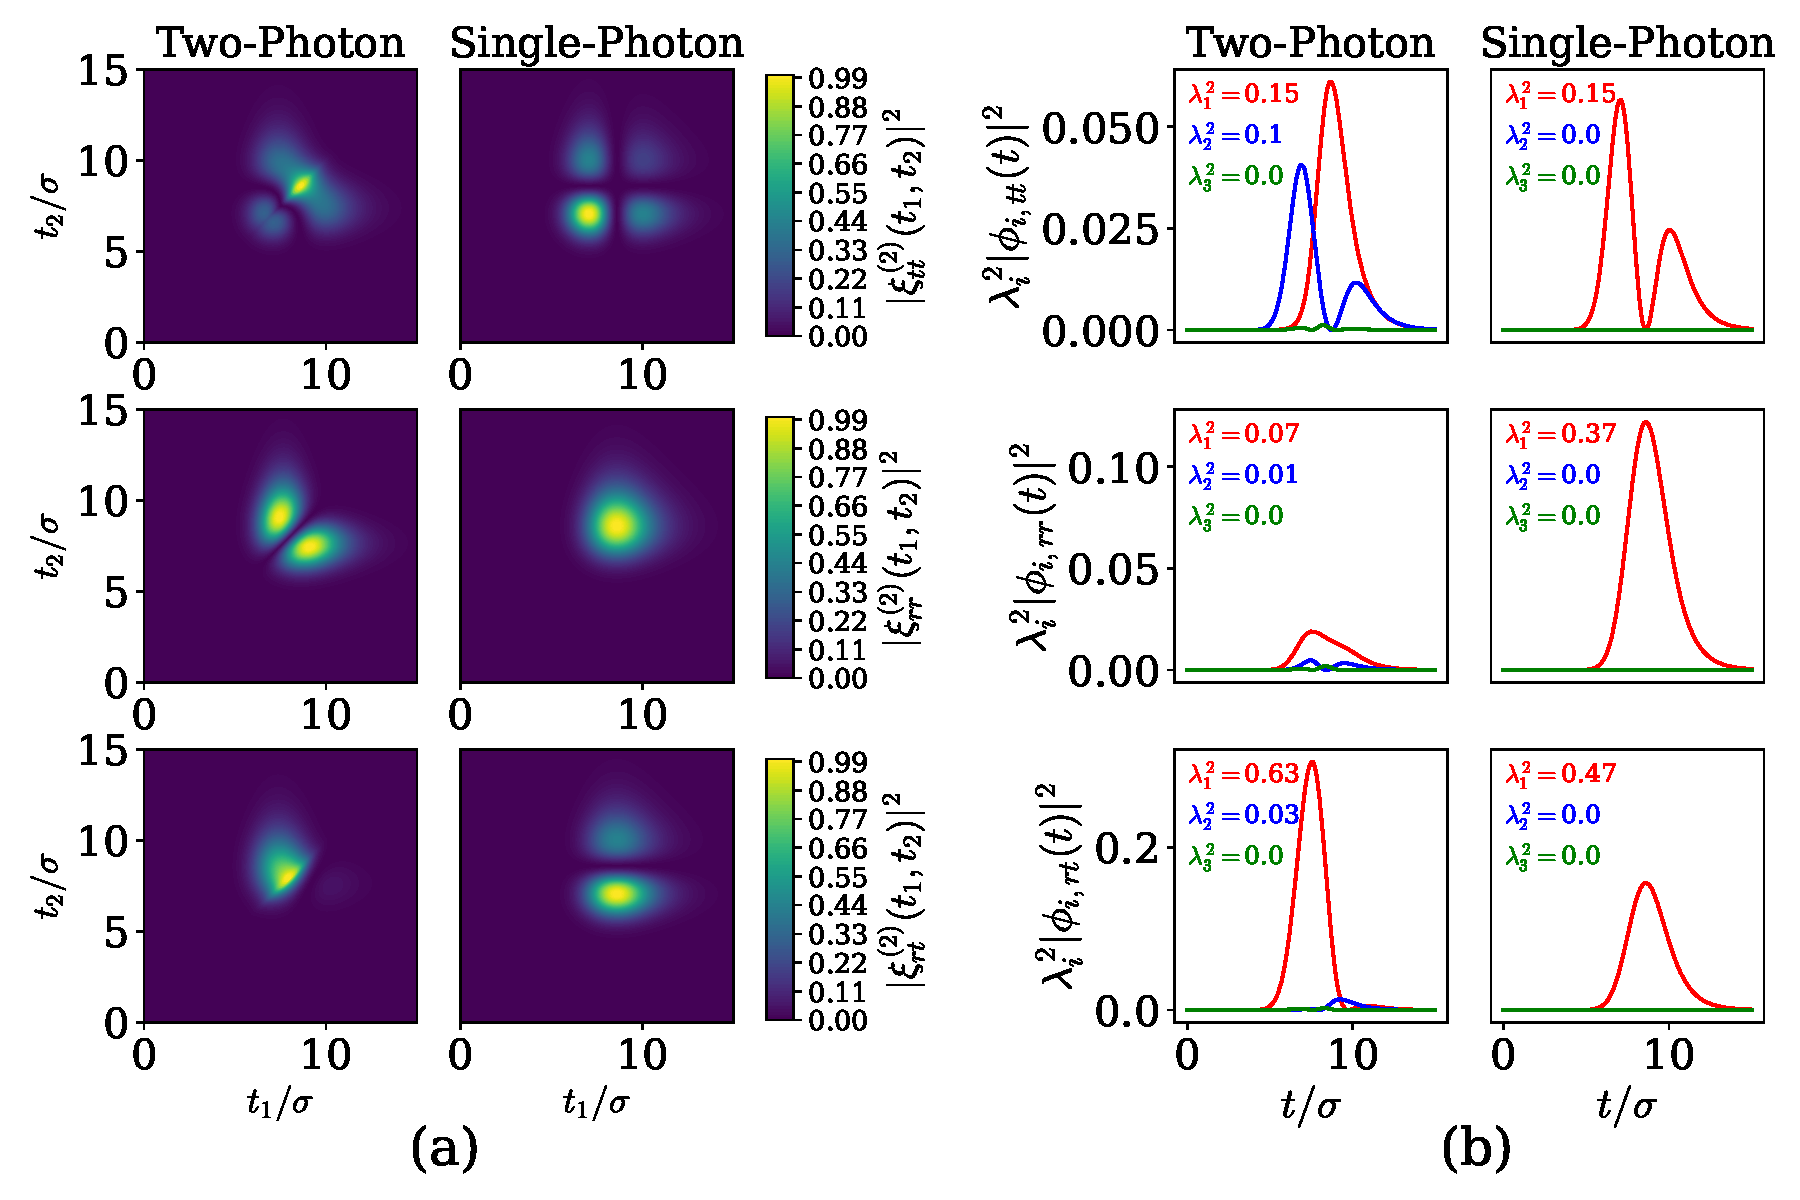
\includegraphics[width=\linewidth]{figures/lodahl_fig3.pdf}
    \caption{(a) Two-photon wavefunctions $\xi^{(2)}_{ij}(t_1,t_2)$ for width $\sigma = 1$ with $\{i,j\} \in \{t,r\}$ describing the wavefunction of both photons being reflected, being transmitted, and one photon being reflected one photon being transmitted, respectively. The left column shows the scattered two-photon wavefunction, while the right shows the single-photon product state $\xi^{(2)}_{ij}(t_1,t_2) = \xi^{(1)}_{i}(t_1)\xi^{(1)}_{j}(t_2)$. All contour plots have been normalized so that the largest value corresponds to unity. (b) The three highest populated modes $\phi(t)$ of the decomposed two-photon wavefunctions. Obviously, the single-photon product state only has one populated decomposed mode $\phi(t)$.}
    \label{fig:lodahlfig3}
\end{figure}

In Fig. \ref{fig:lodahlfig3}, we show the SVD of the wavefunctions and the occupation of the respective decomposed wavefunctions $\phi$. Note that the singular values $\lambda_i^2$ denote the weight of the decomposed function of the total scattered state. Thus $\sum_{i,\mu} \lambda_{i,\mu}^2 = 1$, where $\mu \in \{tt,rr,rt\}$ is the index of the transmitted-transmitted, reflected-reflected, reflected-transmitted state. The single-photon pulse is, by definition, only composed of a single product state, and thus only one relevant orthonormal wavefunction $\phi$ shows up for each scattered wavefunction. For the two-photon case, we see several relevant orthonormal wavefunctions similar to what was seen in ch. \ref{ch3}. The evidence of stimulated emission is seen clearly, as the total population of the two photons being reflected is  significantly reduced with a population of approximately $0.08$ in the two-photon case vs. $0.37$ in the single-photon case, respectively. Similarly, there is an increase in both photons being transmitted with $0.1+0.15 = 0.25$ vs. $0.15$. Also, due to emitter saturation, we see an increase in the first photon being reflected and the second transmitted with $0.67$ vs. $0.48$.







\section{Input Output Relations \label{sec:inputoutput}}
If we now want to consider how waveguide modes can interact directly to form, for example, a partially transmitting element, we now need to define how they interact with each other. In ref. \cite{Xu2016FanoTransport}, they show that fundamental input-output relations can be derived from the Hamiltonian:
\begin{equation}
\begin{aligned}
H= H_{\mathrm{s}}+ \sum_{i=1}^N \int d \nu \hbar \nu w_{i}^{\dagger}(\nu) w_{i}(\nu)+\sum_{i=1}^N \hbar \sqrt{\gamma_i} \int \frac{d \nu}{\sqrt{2 \pi}}\left(w_{i}^{\dagger}(\nu) a+a^{\dagger} w_{i}(\nu)\right) +\sum_{i \neq j} \hbar V_{i j} \int \frac{d \nu}{\sqrt{2 \pi}} \int \frac{d  \nu^{\prime}}{\sqrt{2 \pi}} w_{i}^{\dagger}(\nu) w_{j}(\nu^\prime), \label{eq:generalFAN}
\end{aligned}
\end{equation}
where $w_{i}(\nu)$ is the annihilation operator for waveguide mode $i$ with frequency $\nu$, $\gamma_i$ is the coupling between a local system with Hamiltonian $H_s$ and waveguide mode $i$, and $V_{i,j} =V_{j,i}$ is the unitless coupling between waveguide modes (notice how $d \nu d\nu^\prime w_{i}^{\dagger}(\nu) w_{j}(\nu^\prime)$ has units of inverse time).  As shown in appendix \ref{app:rotating}, we can express the Hamiltonian for time-bin $k$ $H_k$ as :
\begin{equation}
    H_{k} = H_{\mathrm{s}}- \hbar \omega_s a^\dagger a  + \sum_{i=1}^N \hbar \sqrt{\gamma_i/\Delta t} \left(w_{k,i}^{\dagger} a+a^{\dagger} w_{k,i} \right) + \sum_{i \neq j} \hbar  V_{i j}/\Delta t w_{k,i}^{\dagger} w_{k,j} \label{eq:general_transformed}
\end{equation}
where $\omega_s$ is the frequency around which the waveguide pulses are centered. Note, however, that in deriving the above time-bin Hamiltonian we approximated:
\begin{equation}
   \int_{t_{n-1}}^{t_n} dt' w_1^\dagger(t') w_2(t') \approx \frac{1}{\sqrt{\Delta t}} \int_{t_{n-1}}^{t_n} d t' w^\dagger_{1}(t') \frac{1}{\sqrt{\Delta t}} \int_{t_{n-1}}^{t_n} d t' w_{2}(t') =  w^\dagger_{1,n} w_{2,n} \label{eq:interaction_ansatz}
\end{equation}
which is not obvious whether is true. Conceptually, it corresponds to having the two waveguides only interacting at a single point in space and therefore also in time. This is also illustrated in Fig. \ref{fig:beamsplitter_illustration}, where two waveguides interact and form a beamsplitter. In the following, we consider such a configuration and thus no local system ($H_s = 0$). We show that we recover the beamsplitter relations with this Hamiltonian. However, as we shall see, adding a local system, introduces self-energy interactions, which introduces disagreements with the frequency-derived input-output relations. 

Considering two waveguide modes $a$ and $b$ and no local system, the Hamiltonian is:
\begin{equation}
    H_{k,\mathrm{int}} = \hbar V/\Delta t (w_{k,\mathrm{b}}^\dagger w_{k,\mathrm{a}} + w_{k,\mathrm{a}}^\dagger w_{k,\mathrm{b}})
    \label{eq:waveguideinteraction}
\end{equation}
where $w_{k, \mathrm{a} / \mathrm{b}}$ here is the waveguide operator of waveguide $a$ or b at time-bin $k$, and $V$ is the interaction between waveguide $a$ and $b$. 
%After each time-bin has interacted, we thus have the state in the arms after the beamsplitter (here labeled c and d). As we shall see, the strength of $V$ decides the operation of the beamsplitter considered, i.e., whether it is balanced, unbalanced, applies a phase shift, etc.  

The input-output relations for the above interaction can be derived by considering how the operator at time-bin $k$ evolves. Since the Hamiltonian is constant within each time-bin and since we are only interacting with one time-bin at a time, we can write the time-evolution operator for time-bin $k$ as:
\begin{equation}
    U(t_k,t_k+\Delta t) =\exp \left[-\frac{i}{\hbar} \int_{t_k}^{t_k+\Delta t} H_{k,\mathrm{int}} d t^{\prime}\right] = \exp(- i V(w_{k,\mathrm{b}}^\dagger w_{k,\mathrm{a}} + w_{k,\mathrm{a}}^\dagger w_{k,\mathrm{b}} ))
\end{equation}

In the Heisenberg picture, we will thus have the following transformation after the interaction (see appendix \ref{app:waveguideinteraction}):
\begin{equation}
w_{k,\mathrm{a}}(t_k + \Delta t) = U^\dagger(t_k,t_k+\Delta t) w_{k,\mathrm{a}} U(t_k,t_k+\Delta t) = \cos(V) w_{k,\mathrm{a}} - i \sin(V) w_{k,\mathrm{b}}
\end{equation}
Similarly, we have:
\begin{equation}
w_{k,\mathrm{b}}(t_k + \Delta t) = \cos(V) w_{k,\mathrm{b}} - i \sin(V) w_{k,\mathrm{a}}
\end{equation}
This is exactly the beamsplitter transformation \cite{Gerry2004IntroductoryOptics}, and we see that for a 50:50 beamsplitter, we should choose $V_{a,b} = \pi/4$. Note that if we choose instead $H_{k,\mathrm{int}} = \hbar i V/\Delta t (w_{k,\mathrm{b}}^\dagger w_{k,\mathrm{a}} - w_{k,\mathrm{a}}^\dagger w_{k,\mathrm{b}})$, we would instead get (see appendix \ref{app:waveguideinteraction}):
\begin{equation}
w_{k,\mathrm{a}}(t_k + \Delta t) = \cos(V) w_{k,a} - i \sin(V) w_{k,b}
\end{equation}
and:
\begin{equation}
w_{k,\mathrm{b}}(t_k + \Delta t) = \cos(V) w_{k,b} - i \sin(V) w_{k,a}
\end{equation}
which is a similar beamsplitter transformation, but where the beamsplitter applies a different phase. 
\

We can derive similar input-output relations for the more general case where we interact with a quantum system with an arbitrary number of waveguides. We write the general Hamiltonian in eq. \eqref{eq:general_transformed} as: 
\begin{equation}
\begin{aligned}
H_k = H_{s} + H_{k,sb} + H_{k,b} \label{eq:generalinteraction}
\end{aligned}
\end{equation}
where $H_{s}$ is Hamiltonian of the quantum system Hamiltonian, $H_{k,sb} = \sum_{i=1}^N \hbar \sqrt{\gamma_i/\Delta t} \left(w_{k,i}^{\dagger} a+a^{\dagger} w_{k,i} \right)$ the interaction with the system, where $a$ is the annihilation of the quantum system (for a two-level system, $\sigma$ would be a more appropriate symbol), and $\gamma_i$ defines the interaction strength between the quantum system and the corresponding waveguide mode $i$. $ H_{k,b} = \sum_{i \neq j} \hbar  V_{i j}/\Delta t w_{k,i}^{\dagger} w_{k,j}$ defines the interaction between the waveguides modes $i$ and $j$. The time-evolution operator is now given as:
%Note that the form of eq. \eqref{eq:generalinteraction} requires $V_{\mu,\nu} = - V_{\nu,\mu}$ for there to be time-reversal symmetry. In addition, it is shown in ref. \cite{Xu2016FanoTransport} that a Hamiltonian of similar form also ensures flux conservation, energy conservation, and causality.
\begin{equation}
    U(t_k,t_k+\Delta t) =\exp \left[-\frac{i}{\hbar} \int_{t_k}^{t_k+\Delta t} [ H_s + H_{sb} + H_b ] d t^{\prime}\right] = \mathrm{e}^{ \left[ -i \Delta t / \hbar [ H_s + H_{sb} + H_b ] \right ]}
\end{equation}

This form is much more complicated and will, in general, lead to complex self-energy corrections, this is clear if we expand the above exponential using the Zassenhaus formula (in the following we omit a factor of $\Delta t/\hbar$ and absorb it into a normalized Hamiltonian $\Tilde{H} = \Delta t/\hbar H$):

\begin{align}
    U(t_k,t_k+\Delta t) &= \mathrm{e}^{ -i [ \Tilde{H}_s + \Tilde{H}_{sb} + \Tilde{H}_b ]} = \mathrm{e}^{ -i \Tilde{H}_b } \mathrm{e}^{ -i [ \Tilde{H}_{s} + \Tilde{H}_{sb}]} \mathrm{e}^{ 1/2 \comm{\Tilde{H}_b}{\Tilde{H}_{sb}}} \mathrm{e}^{ i/6  \comm{\Tilde{H}_b}{\comm{\Tilde{H}_b}{\Tilde{H}_{sb}}}} \mathrm{e}^{ -1/24 \comm{\comm{\comm{\Tilde{H}_{sb}}{\Tilde{H}_b}}{\Tilde{H}_b}}{\Tilde{H}_b}}\cdots \\
    &= \mathrm{e}^{ -i \Tilde{H}_b } \mathrm{e}^{ -i [ \Tilde{H}_{s} + \Tilde{H}_{sb}]} \mathrm{e}^{-i \Tilde{H}_{eff}} 
\end{align}
where it was used that $\comm{H_b}{H_s} = 0$ and also that $\comm{H_b}{H_{bs}}$ will only generate terms of the type $a w_{k,\mu}^\dagger$ and $a^\dagger w_{k,\mu}$ and so  $\comm{\comm{H_b}{H_{bs}}}{H_{bs}} = 0$. The infinite series will serve as a self-energy correction to the waveguide-system interaction $H_{eff}$, but the input-output relation will still just be given by $\mathrm{e}^{-\Tilde{H_b}}$. The input-output relation can be calculated from the commutator:
\begin{equation}
    \comm{w_{k,\mu}}{H_b} = \sum_{\nu \neq \mu} - i/\Delta t V_{\mu,\nu} w_{k,\nu}
\end{equation}
if we introduce the vector $\textbf{W} = \begin{pmatrix}
    w_{k,1} \\ w_{k,2} \\ \vdots \\ w_{k,N}
\end{pmatrix}$ where $N$ is the number of waveguides, and $\textbf{V} = \begin{pmatrix}
    0 & V_{1,2} & \cdots & V_{1,N} \\
    V_{2,1} & 0 & \cdots & V_{2,N} \\
     \vdots & \vdots & \ddots & \vdots \\
     V_{N,1} & V_{N,2} & \cdots & 0 \\
\end{pmatrix}$ we can write all commutator relations as:
\begin{equation}
    \comm{\textbf{W}}{H_b} = - i/\Delta t \textbf{V} \textbf{W}
\end{equation}
and the waveguide operators thus transform unitary evolution as:
\begin{equation}
    \mathrm{e}^{i \Delta t H_b} \textbf{W} \mathrm{e}^{-i \Delta t H_b} = \textbf{W} + i \Delta t\comm{H_b}{\textbf{W}} - \frac{\Delta t^2}{2!} \comm{H_b}{\comm{H_b}{\textbf{W}}} + \cdots = \textbf{W} + \textbf{V} \textbf{W} + \textbf{V}^2/2! \textbf{W} + \cdots = \exp(\textbf{V}) \textbf{W}  
\end{equation}
and we will thus have the total transformation:
\begin{align}
    U(t_k,t_k+\Delta t)^\dagger \textbf{W} U(t_k,t_k+\Delta t) &=  \mathrm{e}^{i \Tilde{H}_{eff}} \mathrm{e}^{ i [ \Tilde{H}_{s} + \Tilde{H}_{sb}]}  \mathrm{e}^{ i \Tilde{H}_b } \textbf{W} \mathrm{e}^{ -i \Tilde{H}_b } \mathrm{e}^{ -i [ \Tilde{H}_{s} + \Tilde{H}_{sb}]} \mathrm{e}^{-i \Tilde{H}_{eff}} \\
    &= \mathrm{e}^{-i \Tilde{H}_{eff}} \mathrm{e}^{ -i [ \Tilde{H}_{s} + \Tilde{H}_{sb}]}  \exp(\textbf{V}) \textbf{W} \mathrm{e}^{ -i [ \Tilde{H}_{s} + \Tilde{H}_{sb}]} \mathrm{e}^{-i \Tilde{H}_{eff}}
\end{align}
We thus see that if we did not have any local system, the waveguide operators would transform as $\textbf{W}_{out} = \textbf{W}(t+\Delta t) = \textbf{C} \textbf{W}(t)$ with $\textbf{C}=\exp(\textbf{V})$. We here note that the input-output relations calculated from \eqref{eq:generalFAN} in the frequency domain would give \cite{Xu2016FanoTransport}:
\begin{equation}
    \textbf{\textbf{C}} = (\textbf{I} + i\textbf{V}/2)(\textbf{I} + i\textbf{V}/2)^{-1}
\end{equation}
where $\textbf{I}$ is the identity operator and $\textbf{V}$ is as defined above. This means that for two waveguides with arbitrary coupling we would have \cite{Joanesarson2020Few-photonGeometries}:
\begin{equation}
\mathbf{C}=\left(\begin{array}{ll}
t_B & r_B \\
r_B & t_B
\end{array}\right)=\frac{1}{1+\left(\frac{V}{2}\right)^2}\left(\begin{array}{cc}
1-\left(\frac{V}{2}\right)^2 & -i V \\
-i V & 1-\left(\frac{V}{2}\right)^2
\end{array}\right)
\end{equation}
We thus see, that according to this we should choose $V =  2/(1+\sqrt{2})$ to have a balanced beamsplitter. This is obviously different from the above and the discrepancy can most likely be explained by the assumption of eq. \eqref{eq:interaction_ansatz} not being valid. In the following sections, we will investigate this discrepancy and its effect on the accuracy of the simulations. 




With this, we can confirm the derivations of input-output relations in section \ref{sec:inputoutput}. We consider the situation also depicted in Fig. \ref{fig:twowaveguide_illustration}, where we have an initial one-photon Gaussian state in waveguide $a$. We then let waveguide $a$ and $b$ interact with a varying interaction strength $V$ from $0$ to $\pi$ through the Hamiltonian defined in eq. \eqref{eq:waveguideinteraction}. The total population of waveguide $a$ and $b$: $\sum_k \bra{\psi} w_{k,a/b}^\dagger w_{k,a/b} \ket{\psi} $ after the interaction is shown in Fig. \ref{fig:beamsplitter_trans}, and we see that the population of waveguide $a$ follows $\cos(V)^2$ while the population of waveguide $b$ follows $\sin(V)^2$. This is as expected since
\begin{equation}
    \ket{\psi} = \sum_k \sqrt{\Delta t} \xi_a^{(1)}(t_k) \ket{1_k}_a\ket{\emptyset}_b \xrightarrow{BS} \ket{\psi}_{BS} = \sum_k \sqrt{\Delta t} \cos(V) \xi_a^{(1)}(t_k) \ket{1_k}_a\ket{\emptyset}_b - i \sqrt{\Delta t} \sin(V) \xi_a^{(1)}(t_k) \ket{\emptyset}_a\ket{1_k}_b    
\end{equation}
and thus $\sum_k 
\bra{\psi}_{BS} w_{k,a}^\dagger w_{k,a} \ket{\psi}_{BS} = \cos(V)^2 \sum_k \Delta t\abs{\xi_a(t_k)}^2 $ and $\sum_k 
\bra{\psi}_{BS} w_{k,b}^\dagger w_{k,b} \ket{\psi}_{BS} = \sin(V)^2 \sum_k \Delta t \abs{\xi_a(t_k)}^2 $
The code for setting the simulation up is shown in Code Sample \ref{ls:beamsplitter_code}. Here, we create the basis for the efficient representation of multiple waveguides in line 3 and operators associated with waveguides a and b, respectively, in lines 4-7. Finally, we define the initial state in line 10 and solve the evolution in line 11. 



\begin{listing}[H]
\begin{minted}[
frame=lines,
framesep=2mm,
baselinestretch=1.2,
bgcolor=LightGray,
fontsize=\small,
linenos,
escapeinside=||,
mathescape=true
]{julia}
Nphoton = 1 #Number of total excitaitons
NWaveguide = 2#Number of waveguides
bw = WaveguideBasis(Nphoton,Nwaveguide,times)
wda = create(bw,1) #Index 1 for waveguide $a$
wa = destroy(bw,1)
wdb = create(bw,2) #Index 2 for waveguide $b$
wb = destroy(bw,2)
V = pi/4 #pi/4 for balanced beamsplitter
H  = im*V/dt*(wda*wb - wdb*wa)
psi = onephoton(bw,1,xi,times,2,5) #Index 1 to create excitaiton in waveguide $a$
psi_out = waveguide_evolution(times,psi,H) 
\end{minted}
\caption{Code for simulating interactions between two waveguides,}
\label{ls:beamsplitter_code}
\end{listing}

Another example is in Fig. \ref{fig:swapping_twophoton}, where we consider the initial two-photon state in waveguide $a$: $\ket{\psi} = \sum_k \sum_{j \geq k} \Delta t \xi^{(2)}(t_k,t_j) \ket{1_k,1_j}_a\ket{\emptyset}_b$ with $\xi^{(2)}(t_k,t_j) = \xi^{(1)}(t_k)\xi^{(1)}(t_j)$ being a gaussian product state defined in eq. \eqref{eq:gaussian}. Here, we choose $V=\pi/2$ and thus swap the two-photon state from being initially in waveguide $a$ to being in waveguide $b$ after the interaction. 


\begin{figure}
    \centering
    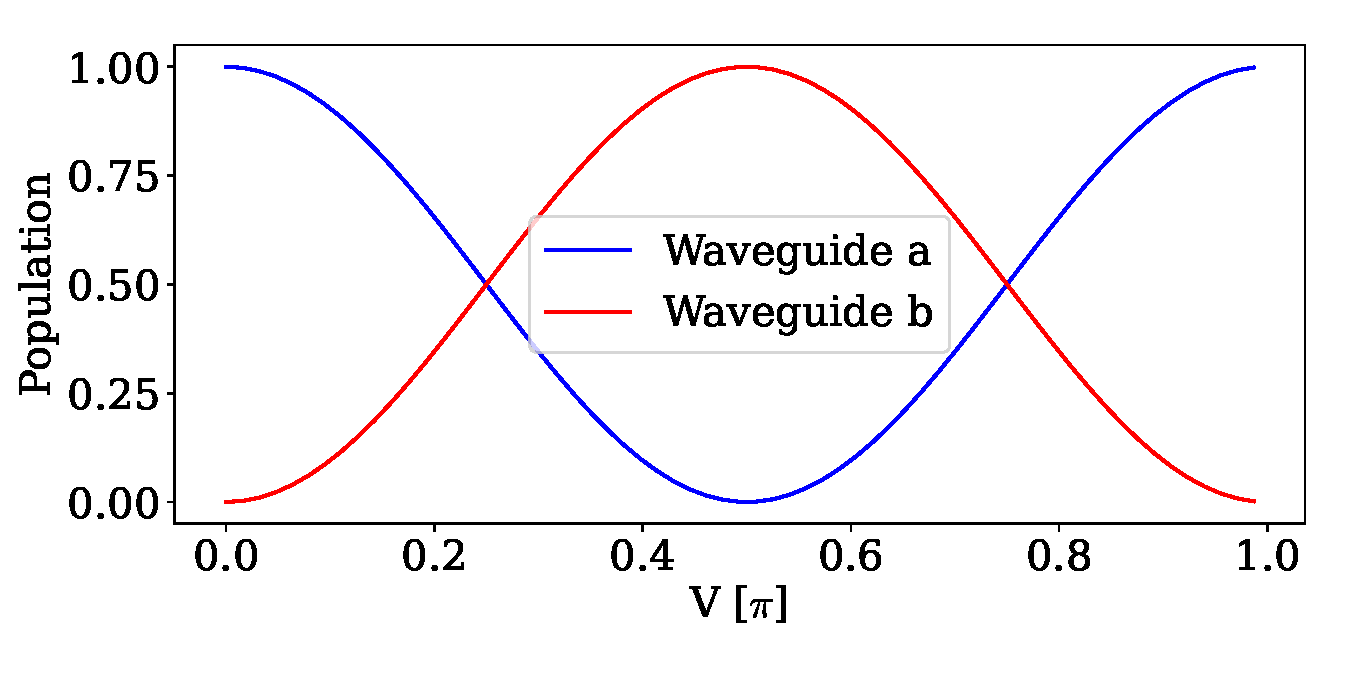
\includegraphics[width=0.6 \linewidth]{figures/beamsplitter_trans.pdf}
    \caption{Population of waveguide $a$ and $b$: $\sum_k \bra{\psi} w_{k,a/b}^\dagger w_{k,a/b} \ket{\psi}$ after interacting for varying coupling strengths $V$. The initial state is a single-photon Gaussian state in waveguide $a$.}
    \label{fig:beamsplitter_trans}
\end{figure}


\begin{figure}[H]
    \centering
    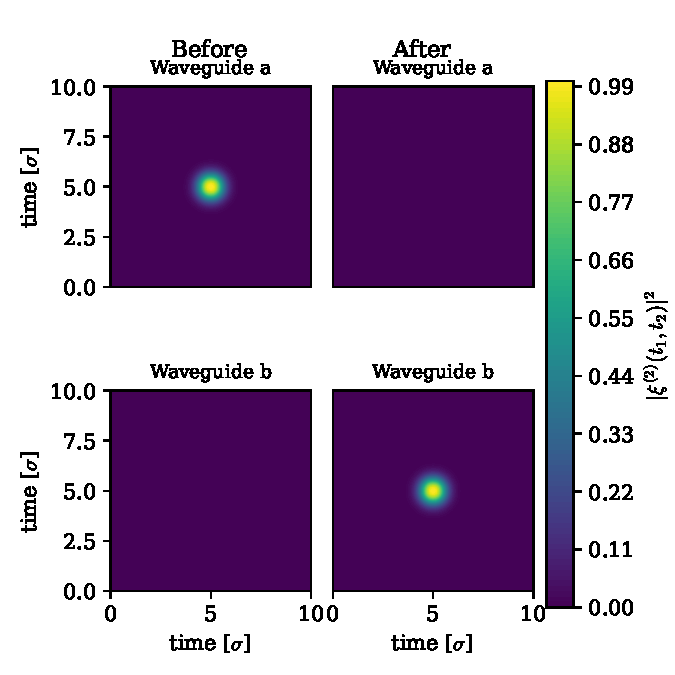
\includegraphics[width=0.6 \linewidth]{figures/swapping_twophoton.pdf}
    \caption{Depiction of two-photon state in waveguide $a$ and $b$, before and after interacting respectively. The initial state is a Gaussian two-photon product state in waveguide $a$, and the interaction strength is $V=\pi/2$ meaning that we swap the excitation from waveguide $a$ to waveguide $b$.}
    \label{fig:swapping_twophoton}
\end{figure}



















\section{Waveguide Interactions \label{sec:waveguideIO}}
We now consider the Hamiltonian in eq. \eqref{eq:lodahl_ham} with $V \neq 0$. $V \neq 0$ can occur due to a defect in the waveguide but also from a purposefully engineered design (such as two terminating waveguides). Either way, an interesting effect of introducing such a defect is a change in the local density of optical states. This can in turn lead to a change in the emitter lifetime \cite{Joanesarson2020Few-photonGeometries}. In ref. \cite{Xu2016FanoTransport}, they derive the input-output relations for the frequency defined Hamiltonian \eqref{eq:generalFAN}:  
\begin{equation}
\begin{gathered}
\frac{d}{d t} a=-i\left[a, H_{\mathrm{c}}\right]-\Sigma a+\mathbf{k}^T \mathbf{W}_{\mathrm{in}} \\
\mathbf{W}_{\text {out }}(t)=\mathbf{C} \mathbf{W}_{\mathrm{in}}(t)+a(t)\mathbf{d}
\end{gathered}
\end{equation}
here $\Sigma$ describes a self-energy correction due to the interaction with the waveguides, and $\mathbf{k}=\mathbf{d}$ is the effective coupling between the waveguides and quantum system. $\mathbf{C}$ was also introduced earlier and defines the direct coupling between the waveguides. All of these relations can be defined in terms of the coupling between the waveguides $\mathbf{V}$ and the coupling between waveguides and the quantum system $\mathbf{\Gamma} = \begin{pmatrix}
    \gamma_1 \\
    \gamma_2 \\
    \vdots \\
    \gamma_N
\end{pmatrix}$ as:
\begin{equation}
\mathbf{C} \equiv\left(\mathbf{I}-\frac{i}{2} \mathbf{V}\right)\left(\mathbf{I}+\frac{i}{2} \mathbf{V}\right)^{-1}, \quad \mathbf{d} = \mathbf{k} \equiv-i\left(\mathbf{I}+\frac{i}{2} \mathbf{V}\right)^{-1} \mathbf{\Gamma}, \quad \Sigma \equiv \frac{1}{2} \mathbf{\Gamma}^T\left(\mathbf{I}+\frac{i}{2} \mathbf{V}\right)^{-1} \mathbf{\Gamma}
\end{equation}
Immediately, it is clear that the interaction between waveguides changes the emitter decay rate as the real part of the self-energy $\Sigma$ describes the decay rate and it depends on the coupling $\mathbf{V}$. If we consider the same configuration as in sec. \ref{sec:lodahl}, we have $\mathbf{\Gamma} = \begin{pmatrix}
    \sqrt{\gamma_L} \\
    \sqrt{\gamma_R} \\
\end{pmatrix}= \begin{pmatrix}
    \sqrt{\gamma/2} \\
    \sqrt{\gamma/2} \\
\end{pmatrix}$ and $\mathbf{V} =\begin{pmatrix}
    0 & V \\
    V & 0 \\
\end{pmatrix}$. This gives the self-energy:
\begin{equation}
    \Sigma = \gamma/2\left( \frac{1}{1+(V/2)^2} - \frac{i V}{2(1+(V/2)^2)} \right) \label{eq:self}
\end{equation}
We see that in the limit of $V=0$ and thus no interacting waveguides, we recover $\Sigma = \gamma/2$ as expected (the emitter population will decay with $\gamma$). For $V \neq 0$ the self-energy also carries an imaginary factor, corresponding to a frequency shift of emitted photons and the decay rate will also be reduced. We can observe this frequency shift and lifetime increase in the emission spectrum of the emitter.

In standard cavity quantum electrodynamics, the emission spectrum of an emitter can be calculated from the Wiener-Kinchen theory and the correlation function \cite{Steck2007QuantumOptics}:
\begin{equation}
    S(\omega) = \gamma\int \int dt d\tau \expval{a^\dagger(t+\tau) a(t)} \mathrm{e}^{-i\tau \omega} \label{eq:wienerkinchen}
\end{equation}
where $a$ here is the cavity annihilation operator and $\gamma$ the coupling to the environment. If we consider an initially excited emitter $\ket{\psi}(0) = \sigma^\dagger \ket{0}$, we will have equal emission into the two waveguides and only have single-photon states of the form $\ket{\psi}(t \rightarrow \infty) = \frac{1}{\sqrt{2}}\left ( \int \xi(t') w_L^\dagger(t') \ket{\emptyset}+\int \xi(t') w_R^\dagger(t') \ket{\emptyset} \right)$. The emission spectrum in either waveguide is then equivalent $S_L(\omega)=S_R(\omega)=S(\omega)$ and is the Fourier transform of the time wavefunction:
\begin{equation}
    S(\omega) = 2 \pi |\xi(\omega)|^2 = \abs{\int dt \xi(t) \mathrm{e}^{-i\omega t}}^2 \label{eq:spec}
\end{equation}
This is evident if we consider no input field since $w_{out}(t) = \sqrt{\gamma} a(t)$ and thus inserting in \ref{eq:wienerkinchen} we get:
\begin{align}
    S(\omega) &= \int \int dt d\tau \expval{w(t+\tau) w(t)} \mathrm{e}^{-i\tau \omega} = \int \int dt d\tau \xi^*(t+\tau) \xi(t) \mathrm{e}^{-i\tau \omega} = \\
    &\frac{1}{2\pi} \int \int \int \int dt d\tau d\omega^\prime d\omega^{\prime \prime} \xi^*(\omega^{\prime}) \xi(\omega^{\prime \prime}) \mathrm{e}^{-i t (\omega^{\prime\prime }-\omega^{\prime}) t} \mathrm{e}^{-i\tau (\omega - \omega^{\prime})} \\
    & = 2 \pi \int \int d\omega^\prime d\omega^{\prime \prime} \xi^*(\omega^{\prime}) \xi(\omega^{\prime \prime}) \delta(\omega^{\prime \prime}-\omega^{\prime})\delta(\omega-\omega^{\prime}) =  2 \pi |\xi(\omega)|^2
\end{align}
\begin{figure}
    \centering
    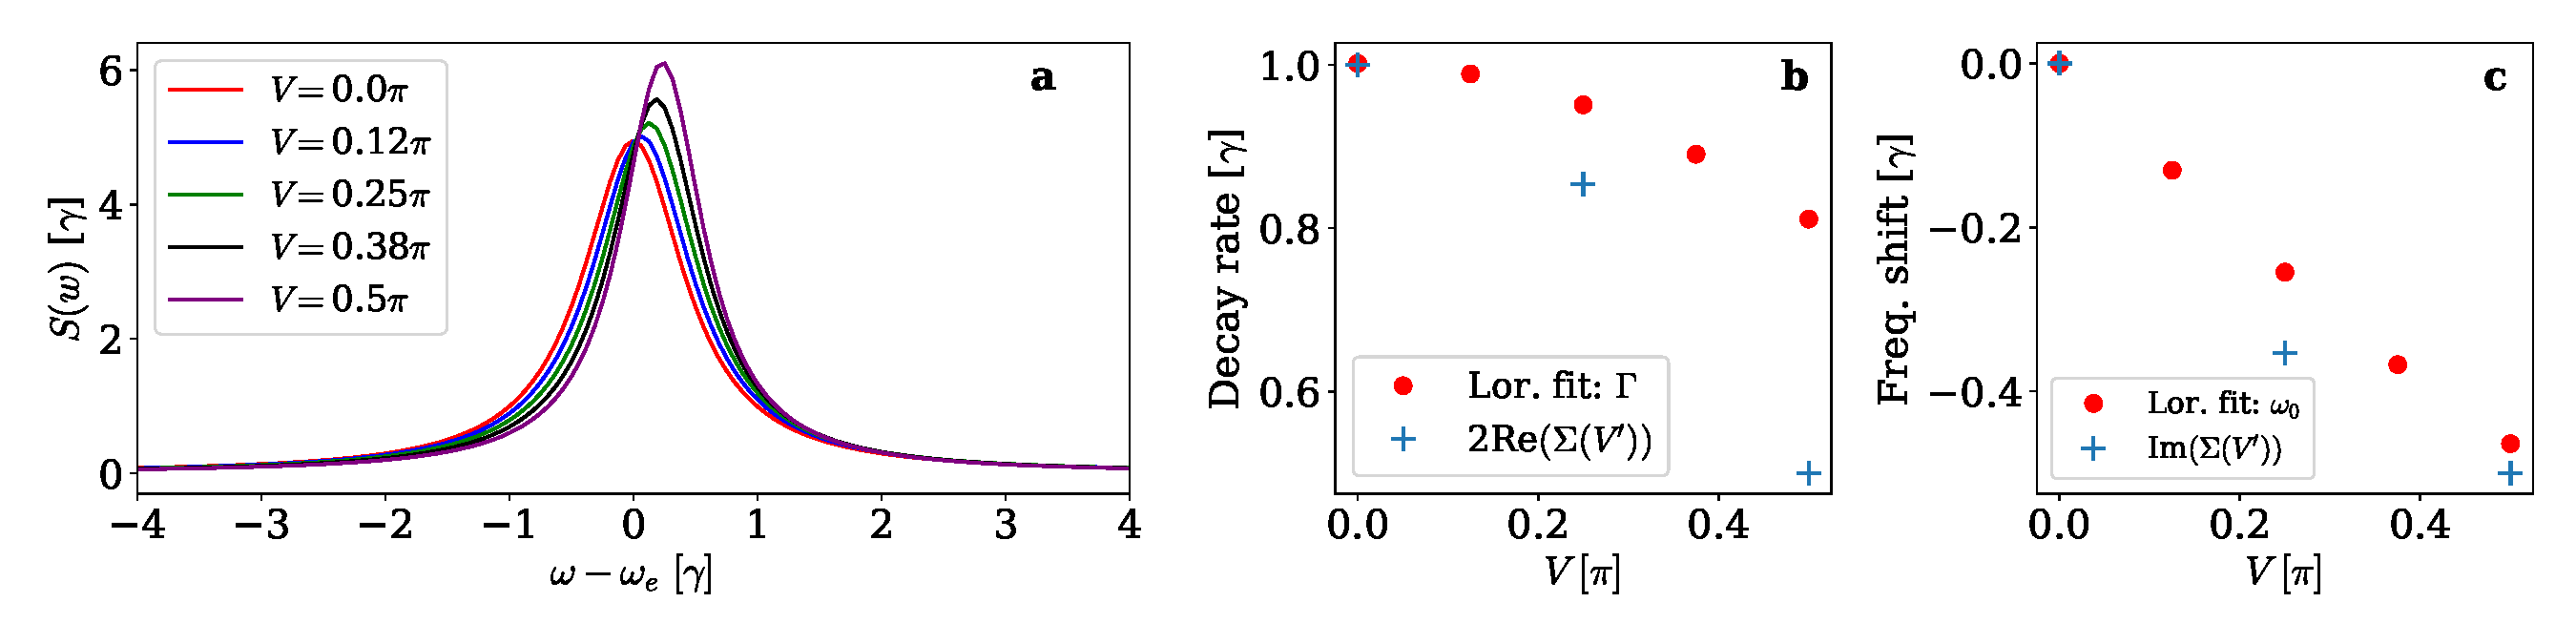
\includegraphics[width=\linewidth]{figures/fanoressonance.pdf}
    \caption{(a) Spectrum as defined in \eqref{eq:spec} for different waveguide couplings $V$. (b) The decay rate (FWHM) of the Lorentzian spectrum in (a) as a function of $V$. The real part of the self-energy $\mathrm{Re}(\Sigma(V'))$ is also plotted for $V'=\{0,2/(1+\sqrt{2}),2\}$ but shown at the points $V =\{0,\pi/4,\pi/2\}$ (for comparison at points with equal input-output relations ). (c) The frequency shift of the Lorentzian in (a) as a function of $V$. $\mathrm{Im}(\Sigma(V'))$ is also shown at the same points as in (b).}
    \label{fig:selfenergy}
\end{figure}


In fig. \ref{fig:selfenergy}(a), we consider the emission spectrum $S(\omega)$ of an initially excited emitter coupled to two waveguides with the same rate $\gamma/2$ and for varying waveguide interaction strength $V$. As $V$ is increased, we see the effect of the waveguide interaction as a shift in the center frequency. The Full Width Half Max (FWHM) which is related to the emitter emission rate is also seen to decrease for larger $V$ as was expected from the change in the self-energy given by eq. \eqref{eq:self}. In fig. \ref{fig:selfenergy} (b)-(c) we plot the FWHM and frequency shift calculated by fitting a Lorentzian on the spectrum in fig. \ref{fig:selfenergy}(a) as a function of $V$. As we established in sec. \ref{sec:inputoutput}, there is not a one-to-one correspondence between the $V$ in ref. \cite{Xu2016FanoTransport} and $V$ in our Hamiltonian in eq. \eqref{eq:lodahl_ham}. Indeed, it was established in sec. \ref{sec:inputoutput} that we should choose $V = \pi/4$ for an even beamsplitter and $V = \pi/2$ for total reflection whereas they find $V=2/(1+\sqrt{2})$ and $V=2$, respectively in ref. \cite{Xu2016FanoTransport}. This discrepancy would be okay as long as the results for the same physical system are the same. For total reflection $V=2$, the self-energy in eq. \eqref{eq:self} predicts an emitter emission rate decrease of $2 \mathrm{Re}(\Sigma(2))/(\gamma/2) = 1/2$, however, as is seen in fig. \ref{fig:selfenergy}, the emission rate is found to decrease by only $\approx 0.8$. A similar, albeit not as large deviation, is also seen in the frequency shift in Fig. \ref{fig:selfenergy}. This shows a fundamental problem with the time-binned picture. The interaction terms $V/\Delta t w_{k,R}^\dagger w_{k,L}$ and $V/\Delta t w_{k,L}^\dagger w_{k,R}$ do not correctly represent the interaction between the waveguides, which is rigorously defined in terms of the frequency Hamiltonian in eq. \eqref{eq:generalFAN}. In the next section, we thus propose another method for handling the input-output relations which does not involve the waveguide interaction terms (and thus $V=0$).

\section{Waveguide Interactions by Rescaling} \label{sec:inferringwaveguide}
Another approach to model the waveguide interactions explicitly with the waveguide interactions $V/\Delta t w_{k,R}^\dagger w_{k,L}$ is to simulate the dynamics without the waveguide interactions and then enforce the input-output relations post-simulation. Indeed, it is argued in ref. \cite{Xu2016FanoTransport} that the system dynamics can be calculated with an effective Hamiltonian $H_{eff} = H_c - i\Sigma a^\dagger a$. In a similar manner, we can omit the waveguide interaction terms if we rescale the waveguide-emitter coupling $\mathbf{\Tilde{\Gamma}} = (\mathbf{I} + \frac{i}{2}\mathbf{V})^{-1} \mathbf{\Gamma}$. Since the emitter-waveguide coupling now can be complex, we have to enforce a Hermitian Hamiltonian by including complex conjugate terms in the coupling:
\begin{equation}
\begin{aligned}
H= H_{\mathrm{s}}+ \sum_{i=1}^N \int d \nu \hbar \nu w_{i}^{\dagger}(\nu) w_{i}(\nu)+\sum_{i=1}^N \hbar \int \frac{d \nu}{\sqrt{2 \pi}}\left(\Tilde{\Gamma}_i^* w_{i}^{\dagger}(\nu) a+ \Tilde{\Gamma}_i a^{\dagger} w_{i}(\nu)\right) \label{eq:modifiedFAN}
\end{aligned}
\end{equation}
where $\Tilde{\Gamma}_i$ is the i'th element of $\Tilde{\mathbf{\Gamma}}$. Notice also that we no longer include waveguide interaction terms in the Hamiltonian. This modification would give a self-energy correction:
\begin{equation}
    \Tilde{\Sigma} = \frac{1}{2} \mathbf{\Tilde{\Gamma}}^\dagger \mathbf{\Tilde{\Gamma}} = \frac{1}{2} \Gamma^T \left ((\mathbf{I} + \frac{i}{2}\mathbf{V})^{-1}\right)^\dagger (\mathbf{I} + \frac{i}{2}\mathbf{V})^{-1} \Gamma = \frac{1}{4}\left (  (\mathbf{I} + \frac{i}{2}\mathbf{V})^{-1} + \left( (\mathbf{I} + \frac{i}{2}\mathbf{V})^{-1}\right)^\dagger \right) = \mathrm{Re}(\Sigma)
\end{equation}
where we used that $C^\dagger = C^*$ and that $(I + i/2 V)^{-1} = 1/2(I+C)$. With the normalized coupling, we thus recover the real part of the self-energy correction. We can then explicitly include the imaginary part by adding a detuning term to our system Hamiltonian: $\Tilde{H_{\mathrm{c}}} = H_{\mathrm{c}} + a^\dagger a \mathrm{Im}(\Sigma)$. With this, the modified input-output relations become:
\begin{align}
& \frac{d}{d t} a= -i\left[a, \Tilde{H_{\mathrm{c}}} \right] -\mathrm{Re}(\Sigma) a + \Tilde{\mathbf{k}}^T \mathbf{W}_{\mathrm{in}} \label{eq:scaledIO1} \\
& \widetilde{\mathbf{W}}_{\text {out }}(t)= \mathbf{\Tilde{C}} \mathbf{W}_{\mathrm{in}}(t)+a(t)\Tilde{\mathbf{d}} \label{eq:scaledIO2}
\end{align}
where $\Tilde{\mathbf{d}} = -i \left(\left(\mathbf{I}+\frac{i}{2} \mathbf{V}\right)^{-1} \right)^* \mathbf{\Gamma}$, $\Tilde{\mathbf{k}} = -i \left(\left(\mathbf{I}+\frac{i}{2} \mathbf{V}\right)^{-1} \right) \mathbf{\Gamma}$, and $\Tilde{\mathbf{C}} = \mathbf{I}$. Eqs. \eqref{eq:scaledIO1} and \eqref{eq:scaledIO2} do, however, not fulfill the constraints that ensure flux conservation time reversal. Specifically, $\Tilde{\mathbf{k}} = \Tilde{\mathbf{d}}$ is not satisfied. This can, however, be restored if we multiply eq. \eqref{eq:scaledIO2} with $\mathbf{C}$ and we thus arrive at:
\begin{align}
\mathbf{C} \widetilde{\mathbf{W}}_{\text {out }}(t)= \mathbf{C} \mathbf{W}_{\mathrm{in}}(t)+a(t)\Tilde{\mathbf{k}}
\end{align}
where we used that $\mathbf{C} \Tilde{\mathbf{d}} = - i/2 \mathbf{C} (\mathbf{I}+\mathbf{C}^*) = \Tilde{\mathbf{k}}$. If we thus define $\mathbf{C} \widetilde{\mathbf{W}}_{\text {out }} \equiv \mathbf{W}_{out}$, we can simulate the dynamics of the system with the rescaled couplings and system Hamiltonian $\Tilde{H}$ but with no waveguide coupling $V=0$, to obtain $\widetilde{\mathbf{W}}_{\text {out }}$. After the simulation, we then apply $\mathbf{C}$ to get $\mathbf{W}_{out}$. Since we are working in the Schr{\o}dinger picture, our output state will be $\ket{\psi}_{\mathrm{out}} = \sum_i \int \widetilde{W}_{out,i}^\dagger \ket{\emptyset}$ and we thus apply $C^\dagger$ to the output state such that: $C^\dagger \ket{\psi}_{\mathrm{out}} = \sum_{i,j} \int C_{i,j}^\dagger \widetilde{W}_{out,i}^\dagger \ket{\emptyset} = \sum_i \int W_{out,i}^\dagger \ket{\emptyset}$. This is shown for a single-photon state but can also be generalized to two-photon states.

\

\begin{figure}
    \centering
    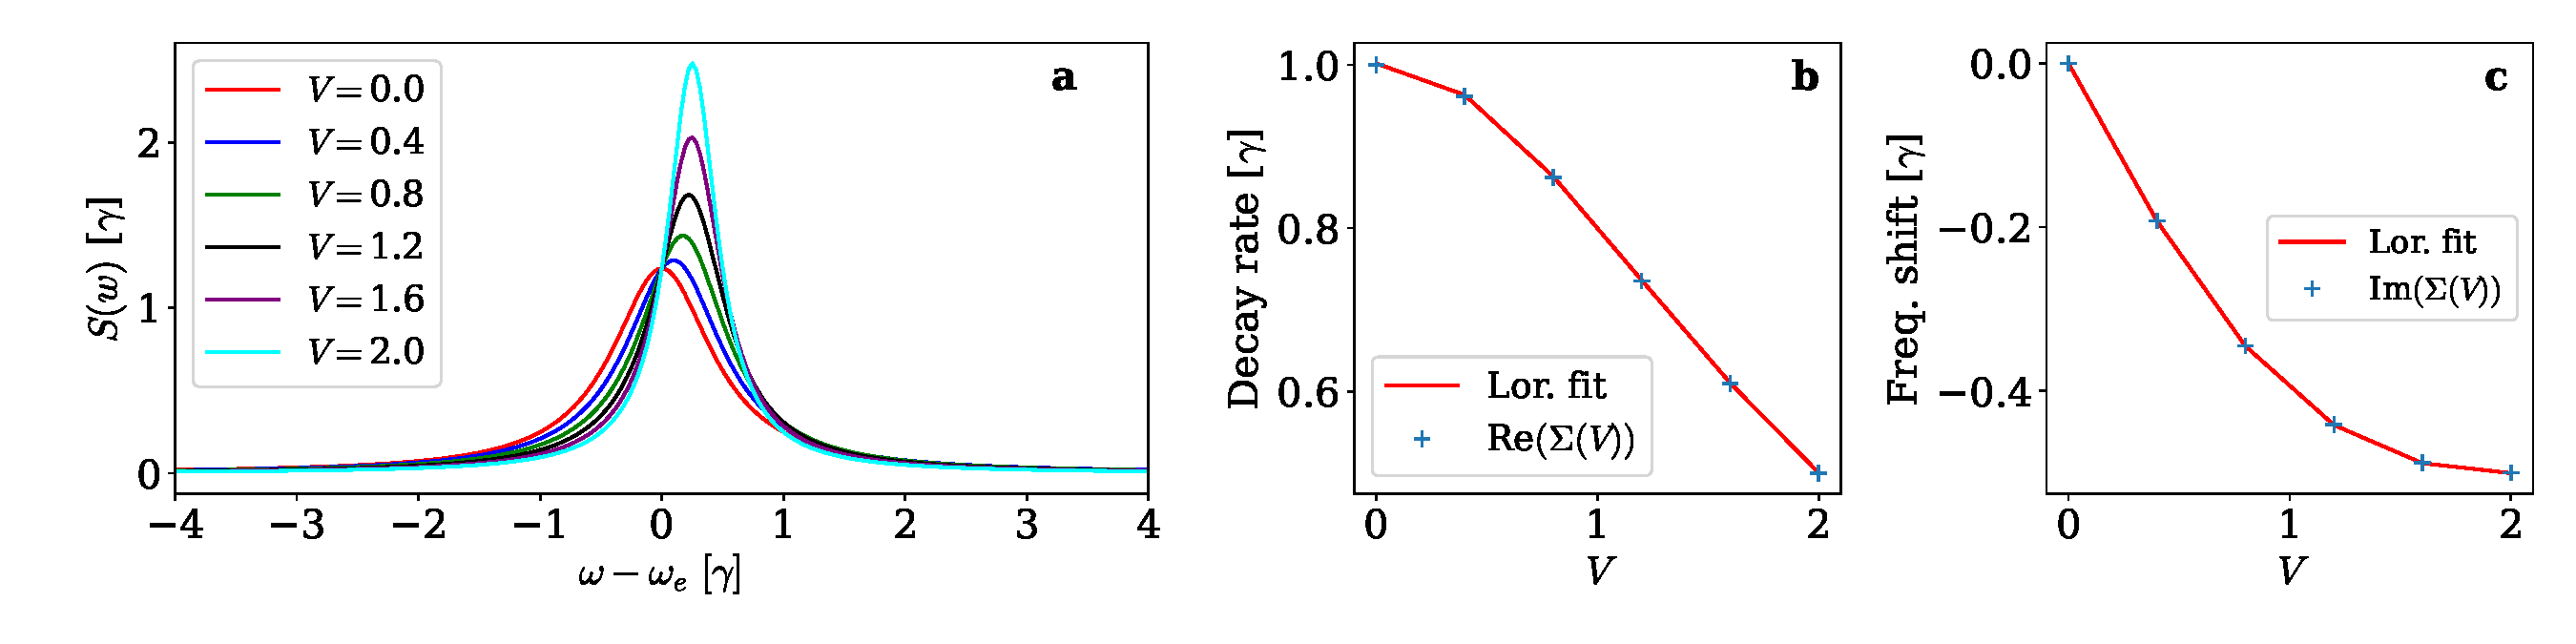
\includegraphics[width = \linewidth]{figures/fanoressonanceIO.pdf}
    \caption{Same as fig. \ref{fig:selfenergy}, but calculated using the rescaling method explained in sec. \ref{sec:inferringwaveguide}}
    \label{fig:DecayIO}
\end{figure}

Using this approach we are able to predict the correct increase in emitter lifetime and shift as is shown in Fig. \ref{fig:DecayIO}. However, this does not prove that we are able to correctly capture the scattering of an incoming. To prove this, we consider how a Gaussian pulse scatters off the emitter for $V=\{0,2/(\sqrt{2}+1),2\}$ corresponding to the case considered in sec. \ref{sec:lodahl}, a 50:50 beamsplitter, and a fully reflecting scattering element. This configuration is also studied in detail in Ref. \cite{Joanesarson2020Few-photonGeometries}. In fig. \ref{fig:fanoIO}, we consider a pulse with a width of $\Tilde{\sigma} = 1.14 (1+(V/2)^2)^{-1}$ corresponding roughly to the pulse width that excites the emitter to the maximum possible probability of 0.4 \cite{Joanesarson2020Few-photonGeometries}. The pulse is also detuned with a frequency of $\Tilde{\omega} = \mathrm{Im}(\Sigma)$ corresponding to the shift in the emitter emission due to the scattering element V. We show the time wavefunction $\xi(t)$, frequency wavefunction $\xi(\omega)$, and the excitation probability as a function of time. We see that except for different widths of the emitted field, $V=0$ and $V=2$ are the same, except that the transmitted and reflected fields are swapped. In the case of a beamsplitter $V=2/(1+\sqrt{2})$, the output fields are asymmetric in frequency space, but with the same excitation probability of exactly 0.5.   

\begin{figure}
    \centering
    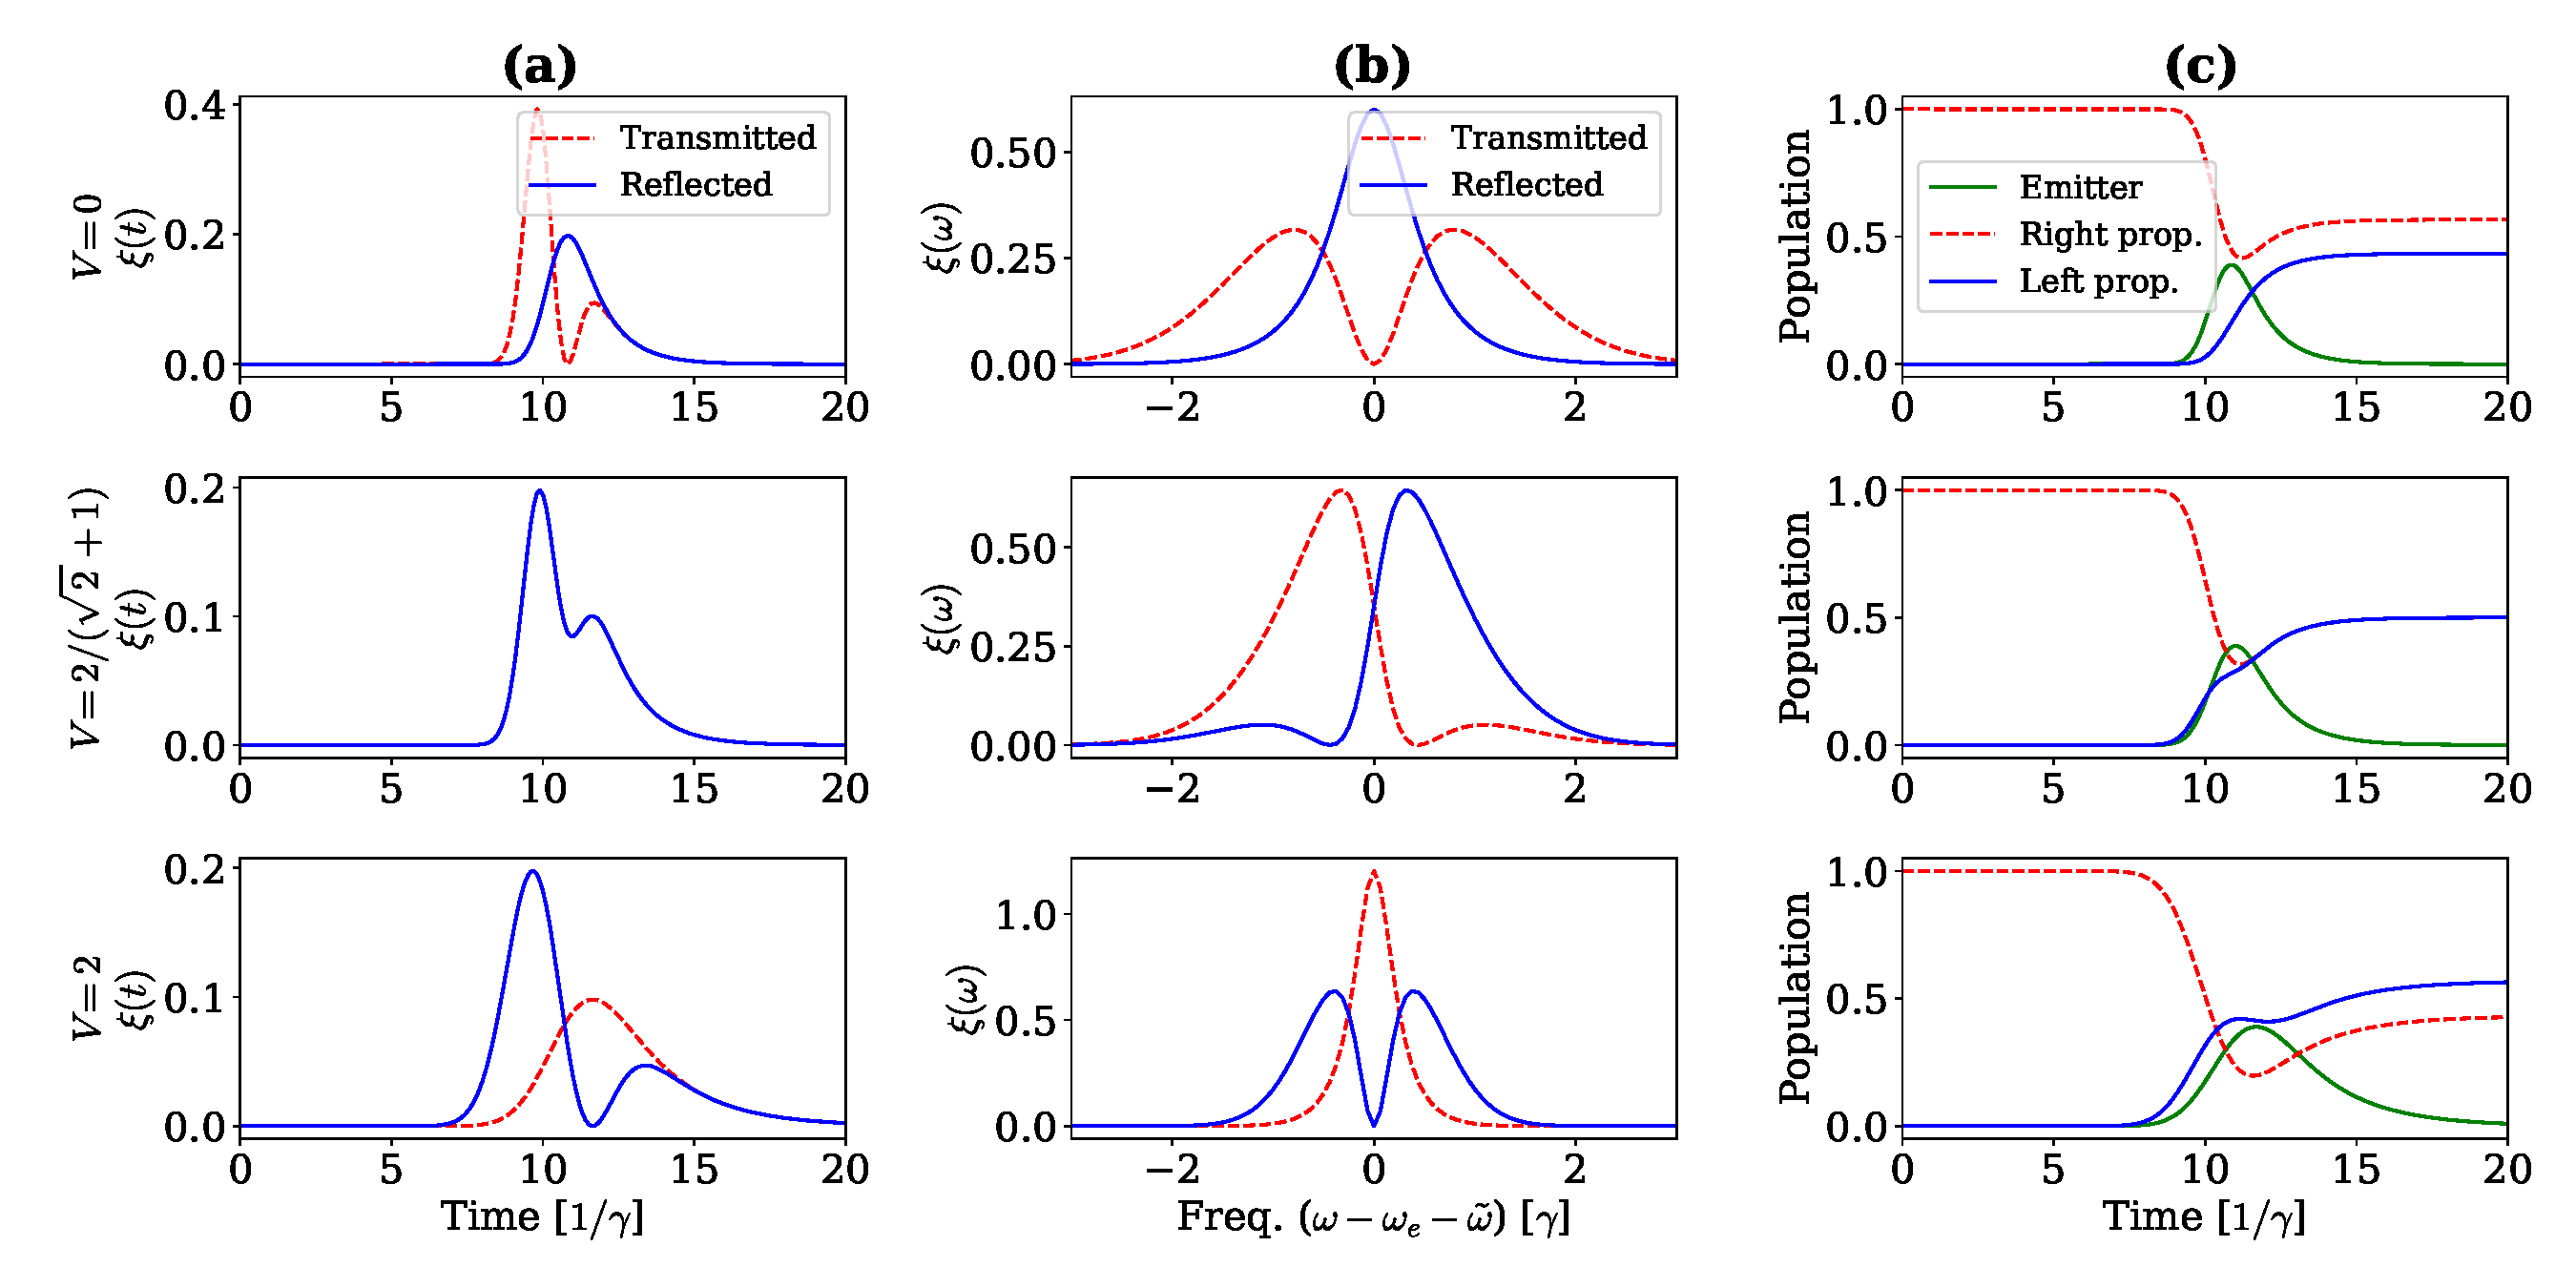
\includegraphics[width=\linewidth]{figures/Fanoscattering.pdf}
    \caption{Column (a): The time-wavefunction $\xi(t)$ as a function of time. Column (b) The frequency wavefunction $\xi(\omega)$, notice that the frequency axis is shifted with the frequency $\Tilde{\omega} = \mathrm{Im}(\Sigma)$ arising from the waveguide interactions. Column (c) the population of the emitter, left, and right propagating fields. The first row shows the case of $V=0$ corresponding to no scattering element, the second row shows $V=2/(1+\sqrt{2})$ corresponding to a beamsplitter, and the third row $V=2$ corresponding to a fully reflecting element.  }
    \label{fig:fanoIO}
\end{figure}





